\documentclass{article}
\usepackage[utf8]{inputenc}
\usepackage{amsmath,amssymb,amsfonts,amsthm,graphicx,enumitem,algorithm,algorithmic}
\usepackage{caption}
\usepackage{subcaption}
\usepackage[parfill]{parskip}
\usepackage{mathrsfs}
\DeclareMathOperator*{\argmin}{arg\,min}
\DeclareMathOperator*{\argmax}{arg\,max}
\usepackage[top=1in,bottom=1in,left=1.4in,right=1.4in]{geometry}

\title{ \vspace{-5mm}
        Probabilistic Graphical Models 10-708\\
        Homework 3}         % <-- Edit Homework Number
\author{Daniel Ribeiro Silva\\      % <-- Edit Name
Andrew ID: drsilva}        % <-- Edit Andrew Id

\begin{document}
\maketitle


% -------------------------------------------------------
%       Problem 1
% -------------------------------------------------------

\section*{Problem 1}


% Part 1
% -------
\subsection*{Part 1}

\begin{enumerate}

% 1
% ---
\item
Friends network structure\\

\begin{enumerate}
%1.a
\item
It is important to notice that in this problem we want to assess the structure of a graph, but the random variables are the edges and not the nodes. 
\begin{itemize}
\item
$Y_{ij,t}$ is the friendship status between students $i$ and $j$ at the time during homework $t$.
This is a binary variable: 0 for ``friendship exists'' and 1 for ``friendship doesn't exist''
\item
$X_{ij,t}$ is the homework similarity between students $i$ and $j$ for homework $t$.
This is a categorical variable, representing the level of similarity. We could define something like 3 or 4 levels of similarity.
\end{itemize}
%1.b
\item
We have one generative model for each friendship $ij$ which is modelled by a HMM such that:
\begin{itemize}
\item 
$P(Y_{ij,t}|X_{ij,1:t-1},Y_{ij,1:t-1}) = P(Y_{ij,t}|Y_{ij,t-1})$ 
\item
$P(X_{ij,t}|X_{ij,1:t-1},Y_{ij,1:t}) = P(X_{ij,t}|Y_{ij,1:t})$
\end{itemize}
%1.c
\item Graphical model: Figure \ref{graphmodelone}
\begin{figure}[ht!]
\centering
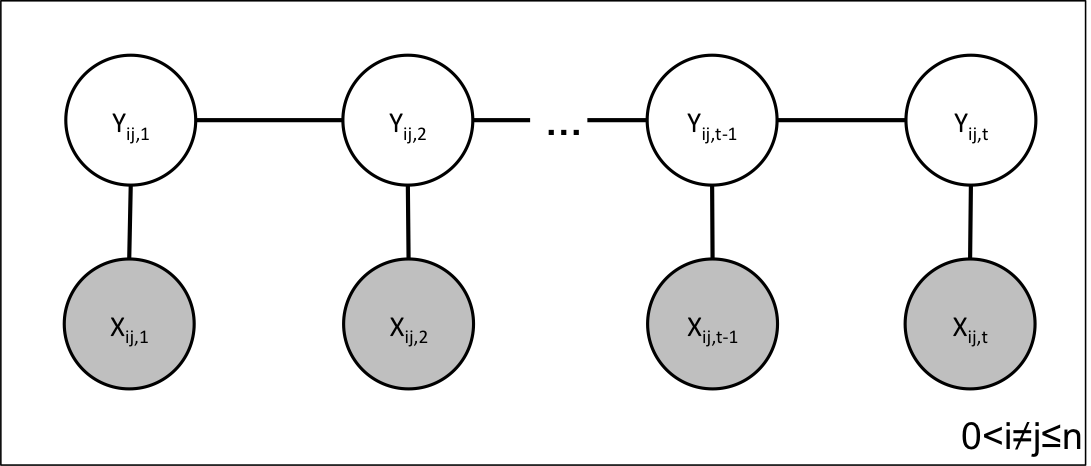
\includegraphics[width=90mm]{1_1_1.png}
\caption{Graphical model corresponding to the proposed model}
\label{graphmodelone}
\end{figure}
%1.d
\item
For each possible edge $ij$ and for each moment/time $t$ we want to find out the probability that they are friends: $P(Y_{ij,t})$. This can be assessed from the joint probability of this variable and the data $P(Y_{ij,t},X_{ij,1:T})$ or from the conditional probability of that variable given the data $P(Y_{ij,t}|X_{ij,1:T})$, where $T$ is the total number of homeworks. By knowing the value of this probability, one is able to assess how strong the friendship between the two students is at that moment of time, and this is the key information we need to propose the construction of a friendship graph. A simple approach would be to establish an empirical threshold on the probability such that if the probability is larger than the threshold, then we assume that the friendship exists (edge exists). Otherwise, we assume the friendship doesn't exist.
%1.e
\item
Possible inference algorithms for this problem are the Viterbi algorithm and the Forward-Backward algorithm. Transition and emission matrices could be generated using human intuition of the problem or learned form labeled data.
\end{enumerate}



% 2
\item
Animal communities assessement\\

\begin{enumerate}
%1.a
\item
It is important to notice that in computer vision/image analysis it is usually a very bad idea to work with the pixel granularity. So my suggestion for this specific problem would be to use specific image descriptors instead of pixel information. In specific, I believe a combination of SIFT and Color Descriptors could be an interesting solution for the feature modelling of this specific problem. My solution for this problem would be to use a topic model approach based on Latent Dirichlet Allocation (LDA) with the images corresponding to the documents, the animals corresponding to the topics, and the image features (originated from the image descriptors) corresponding to the words. So for our variables we will use the same notation from \cite{lda}:
\begin{itemize}
\item
$\theta$: random variable that corresponds to the multinomial parameter for the topic selection of a given word. More precisely, we can write $\theta = \theta_{d,n}$ as being the multinomial parameter for the topic selection for the $n$-th word of the $d$-th document.
\item
$z$: corresponds to the topic selected for a given word of a document. More precisely, we can write $z = z_{d,n}$ as being the topic for the $n$-th word of the $d$-th document.
\item
$w$: the selected word conditional to the previously selected topic $z$. More precisely, we can write $w = w_{d,n}$ as being the $n$-th word of the $d$-th document.

\end{itemize}
%1.b
\item
The generative model is given by:
\begin{enumerate}
\item For each image (document) $d$ on the stack, use SIFT and Color descriptors to extract high-level features.
\item Choose $\theta \sim Dir(\alpha)$. The dimensionality of the $Dir$ distribution is 200 (number of animals/topics).
\item For each of the N extracted features (words) $w_n$:
\begin{enumerate}
\item Choose an animal (topic) $z_n \sim Multinomial(\theta)$.
\item Choose a feature (word) $w_n$ from $p(w_n|z_n,\beta)$, a multinomial probability conditioned on the topic $z_n$.
\end{enumerate}
\end{enumerate}

%1.c
\item 
Original graphical model: Figure \ref{graphmodeltwo}
\begin{figure}[ht!]
\centering
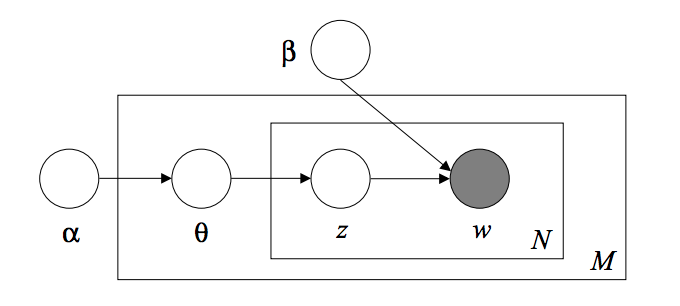
\includegraphics[width=90mm]{1_1_2.png}
\caption{Graphical model corresponding to the proposed model}
\label{graphmodeltwo}
\end{figure}
Adapted graphical model used for inference: Figure \ref{graphmodeltwoprime}
\begin{figure}[ht!]
\centering
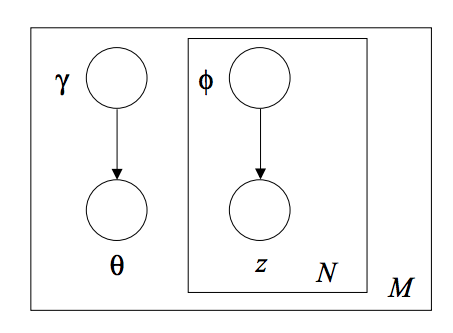
\includegraphics[width=90mm]{1_1_2b.png}
\caption{Graphical model corresponding to the adapted model for inference}
\label{graphmodeltwoprime}
\end{figure}
%1.d
\item
First of all, the quantity we want to infer is the posterior distribution of the hidden variables ($\theta$ and $z$, which represent the variables associated with the topic) given a document (the words on that document):
\begin{equation*}
p(\theta,z|w,\alpha,\beta) = \frac{p(\theta,z,w|\alpha,\beta)}{p(w|\alpha,\beta)}
\end{equation*}
With information about $\theta$, we can assess, for each document (image), what are its most representative topics. We can then build a matrix $M$ with $D$ rows and $200$ columns, where each element $M_{i,j}$ represents a centred and normalized representativeness of the topic (animal) $j$ on the document $i$.
If we compute the covariance matrix $N = M^TM$, we obtain a symmetric matrix that contains information about the appearance correlation of different animals on the photo dataset. Basically, if the element $N_{i,j}$ has a high value, it means that animals $i$ and $j$ tend to appear on the same photo (and therefore coexist in the same habitat).
%1.e
\item
We can use the variational inference algorithm presented in \cite{lda}. This algorithm makes small changes on the graphical model to make the inference problem tractable. The new graphical model used for the inference problem is given by Figure \ref{graphmodeltwoprime}. The inference algorithm \cite{lda} is given by:
\begin{figure}[ht!]
\centering
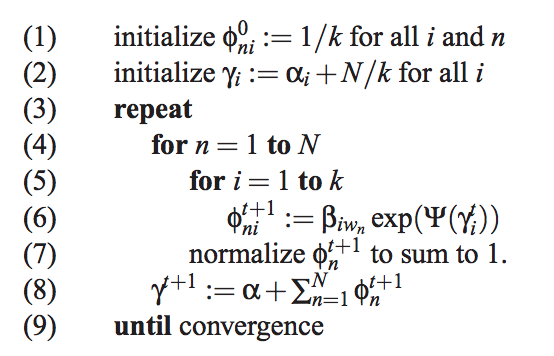
\includegraphics[width=75mm]{1_1_2inf.png}
\caption{Variational inference algorithm}
\label{varinfalgorithm}
\end{figure}

\end{enumerate}

\end{enumerate}

\newpage
% Part 2
% -------
\subsection*{Part 2}

\begin{enumerate}
% 1
\item
It is preferable to use HMMs in the case where the hidden variables assume discrete values (LDS assumes continuous values) and when the learning is unsupervised/no labeled data is available (CRF assumes supervised learning).
Example of applications include trend prediction in the financial market (as seen in the previous assignment).
% 2
\item
It is preferable to use CRF when we have labeled data and also when it is hard to model the data $P(x)$ (or when we don't wish to), since CRF only uses $p(y|x)$. That is not the case for HMM or LDS. 
Example of applications for CRF include shallow parsing and pattern recognition in computer vision.
% 3
\item
It is preferable to use LDS in the case where the hidden variables assume continuous values (HMM assumes discrete values) and when the learning is unsupervised/no labeled data is available (CRF assumes supervised learning). 
Example of applications include continuous dynamical phenomena such as human motion or maneuvering targets.
% 4
\item
For LDS we can use the forward and the backward update in a very similar way as we do for HMM, but now we have to consider that the hidden variables are continuous, which means that the update equations will no longer be a sum, but an integral over the values, as follows:
\begin{equation*}
\alpha(y_t) = \int p(x_t|y_t)p(y_t|y_{t-1})\alpha(z_{t-1})dz_{t-1}
\end{equation*}

\begin{equation*}
\beta(y_t) = \int p(x_{t+1}|y_{t+1})p(y_{t+1}|y_t)\beta(z_{t+1})dz_{t+1}
\end{equation*}
% 5
\item
As it is explained on Question 3 - Item 3, we can use the forward-backward algorithm as a form of message-passing to compute the probability $P(y_i, y_{i+1}, \dots, y_{i+k} | {\bf x})$ by doing

\begin{equation*}
P(y_i, y_{i+1}, \dots, y_{i+k} | | {\bf x}) = \frac{1}{Z(x)}\alpha_{i-1} \prod_{j=i}^{i+k} M_j(y_j, y_{j-1}) \beta_{i+k}^T
\end{equation*}

Please refer to Question 3 - Item 3 for the detailed explanation.

\end{enumerate}


\newpage
% -------------------------------------------------------
%       Problem 2 
% -------------------------------------------------------

\section*{Problem 2}

\begin{enumerate}

% 1
\item
If all the variables were observed, the conditional log-likelihood of the data would be given by
\begin{equation*}
l(\theta;x,y,z) = \log p(y,z|x,\theta;\sigma^2, \gamma)
\end{equation*}

But singe, $z$ is unobserved, the conditional likelihood must be expressed as a marginal probability over that hidden variable 
\begin{equation*}
l(\theta;x,y) = \log \sum_{z}p(y,z|x,\theta;\sigma^2, \gamma)
\end{equation*}

We multiply that expression by $1 = \frac{p(z|x,y;\gamma)}{p(z|x,y;\gamma)}$  
\begin{equation*}
l(\theta;x,y) = \log \sum_{z}\frac{p(z|x,y;\gamma)}{p(z|x,y;\gamma)}p(y,z|x,\theta;\sigma^2, \gamma) = \log \sum_{z}p(z|x,y;\gamma)\frac{p(y,z|x,\theta;\sigma^2, \gamma)}{p(z|x,y;\gamma)}
\end{equation*}

Since the log function is a concave function, we can use Jensen's inequality to get
\begin{equation*}
l(\theta;x,y) = \log \sum_{z}p(z|x,y;\gamma)\frac{p(y,z|x,\theta;\sigma^2, \gamma)}{p(z|x,y;\gamma)} \ge \sum_{z}p(z|x,y;\gamma)\log\frac{p(y,z|x,\theta;\sigma^2, \gamma)}{p(z|x,y;\gamma)}
\end{equation*}

This can be rewritten as 
\begin{equation*}
l(\theta;x,y) \ge \sum_{z}p(z|x,y;\gamma)\log p(y,z|x,\theta;\sigma^2, \gamma) - \sum_{z}p(z|x,y;\gamma)\log{p(z|x,y;\gamma)}
\end{equation*}

We start by observing that we ca use Bayes theorem to write $p(y,z|x,\theta;\sigma^2, \gamma) = p(y|x,z;\theta,\sigma^2)p(z|x;\gamma)$, which gives us
\begin{equation*}
l(\theta;x,y) \ge \sum_{z}p(z|x,y;\gamma)\log p(y|x,z;\theta,\sigma^2) + \sum_{z}p(z|x,y;\gamma)\log p(z|x;\gamma) - \sum_{z}p(z|x,y;\gamma)\log{p(z|x,y;\gamma)}
\end{equation*}

Finally, we observe that $-\sum_{z}p(z|x,y;\gamma)\log{p(z|x,y;\gamma)}$ is the entropy, which is independent of $\theta$ and which is always bigger or equal than $0$ (observe we include the minus sign on the term). We call this term $\mathcal{H}_p(z|x,y)$. We then get
\begin{equation*}
\begin{split}
l(\theta;x,y) &\ge \sum_{z}p(z|x,y;\gamma)\log p(y|x,z;\theta,\sigma^2) + \sum_{z}p(z|x,y;\gamma)\log p(z|x;\gamma) + \mathcal{H}_p(z|x,y)\\
&\ge \sum_{z}p(z|x,y;\gamma)\log p(y|x,z;\theta,\sigma^2) + \sum_{z}p(z|x,y;\gamma)\log p(z|x;\gamma)
\end{split}
\end{equation*}

By the definition of the expectation according on a probability, we can rewrite it as
\begin{equation*}
l(\theta;x,y) \ge \mathbb{E}_{p(z|x,y)}\left[\log p(y|x,z;\theta,\sigma^2)\right] + \mathbb{E}_{p(z|x,y)}\left[\log p(z|x;\gamma)\right]
\end{equation*}

If we want to write it in terms of the data instances, we use the linearity of the expectation function and the independence of the instances. We obtain
\begin{equation*}
l(\theta;x,y) \ge \sum_{n=1}^N\mathbb{E}_{p(z|x,y)}\left[\log p(y_n|x_n,z_{nk};\theta_k,\sigma_k^2)\right] + \sum_{n=1}^N\mathbb{E}_{p(z|x,y)}\left[\log p(z_{nk}|x_n;\gamma_k)\right]
\end{equation*}



%2
\item EM Steps:

\subsubsection*{E-Step}
We want to compute the value of $p(z|x,y)$ for a given $\theta$.
\begin{equation*}
\begin{split}
\tau_n^k = p(z_{nk}=1|x_n,y_n,\theta^{(t)}) &= \frac{p(z_{nk}=1,x_n,y_n|\theta^{(t)})}{p(x_n,y_n|\theta^{(t)})}\\
&=\frac{p(z_{nk}=1|x_n)p(y_n|x_n,\theta_k^{(t)},\sigma_k^2)}{\sum_j p(z_{nj}=1|x_n)p(y_n|x_n,\theta_j^{(t)},\sigma_j^2)}
\end{split}
\end{equation*}

The first step is just Bayes rule and the second step is derived from the structure of the probabilistic graphic model and form marginalising over $z$.

\subsubsection*{M-Step}
We wish to find the $\theta$ that maximizes the likelihood of the objective function for a fixed $p(z|x,y)$. By taking the derivative of the objective function w.r.t. $\theta$ we get:

\begin{equation*}
\begin{split}
\frac{\partial}{\partial \theta}l(\theta;x,y) &= \frac{\partial}{\partial \theta}\sum_{n=1}^N\mathbb{E}_{p(z|x,y)}\left[\log p(y_n|x_n,z_{nk};\theta_k,\sigma_k^2)\right] + \frac{\partial}{\partial \theta}\sum_{n=1}^N\mathbb{E}_{p(z|x,y)}\left[\log p(z_{nk}|x_n;\gamma_k)\right]\\
 &= \frac{\partial}{\partial \theta}\sum_{n=1}^N\mathbb{E}_{p(z|x,y)}\left[\log p(y_n|x_n,z_{nk};\theta_k,\sigma_k^2)\right] = 0\\
\end{split}
\end{equation*}

That implies 

\begin{equation*}
\frac{\partial}{\partial \theta}\sum_{n=1}^N\sum_{k=1}^K \tau_n^k\log p(y_n|x_n,z_{nk};\theta_k,\sigma_k^2) = 0\\
\end{equation*}

But we know that

\begin{equation*}
Y_n | X_n = x_n, Z_n = k \sim Normal(\theta_k^T x_n, \sigma_k^2)
\end{equation*}

Thus,
\begin{equation*}
\begin{split}
\frac{\partial}{\partial \theta}\sum_{n=1}^N\sum_{k=1}^K \tau_n^k\log p(y_n|x_n,z_{nk};\theta_k,\sigma_k^2) &= \frac{\partial}{\partial \theta}\sum_{n=1}^N\sum_{k=1}^K \tau_n^k \left( -\log(\sqrt{2\pi}) - \log(\sigma_k) + \frac{(y_n-\theta_k^Tx_n)^2}{2\sigma_k^2}  \right)\\
&= \frac{1}{2\sigma_k^2}\frac{\partial}{\partial \theta}\sum_{n=1}^N\sum_{k=1}^K \tau_n^k  (y_n-\theta_k^Tx_n)^2\\
&= \frac{1}{2\sigma_k^2}\frac{\partial}{\partial \theta}\sum_{n=1}^N  (Y-\theta X)^TT(Y-\theta X) = 0\\
\end{split}
\end{equation*}

Where $T = \sum_{n=1}^Ndiag(\tau_n^1,\dots,\tau_n^K)$

Thus,

\begin{equation*}
\frac{\partial}{\partial \theta} (Y-\theta X)^TT(Y-\theta X) = 0\\
\end{equation*}

By expanding the expression, merging equal terms and removing terms independent of $\theta$, we get

\begin{equation*}
\frac{\partial}{\partial \theta}  X^T\theta^TT\theta X - 2Y^TT\theta X = 0\\
\end{equation*}

If we take the derivative, we get:

\begin{equation*}
2X^TTX\theta - 2X^TTY = 0\\
\end{equation*}

Finally, we obtain our $\theta$:

\begin{equation*}
\theta = (X^TTX)^{-1}X^TTY\\
\end{equation*}

\end{enumerate}

\newpage
% -------------------------------------------------------
%       Problem 3 
% -------------------------------------------------------

\section*{Problem 3}

\begin{enumerate}

% 1
\item
The graphical model corresponding to the conditional distribution of equation (1) on the handout is given by Figure \ref{meanfieldmodel}\\

\begin{figure}[ht!]
\centering
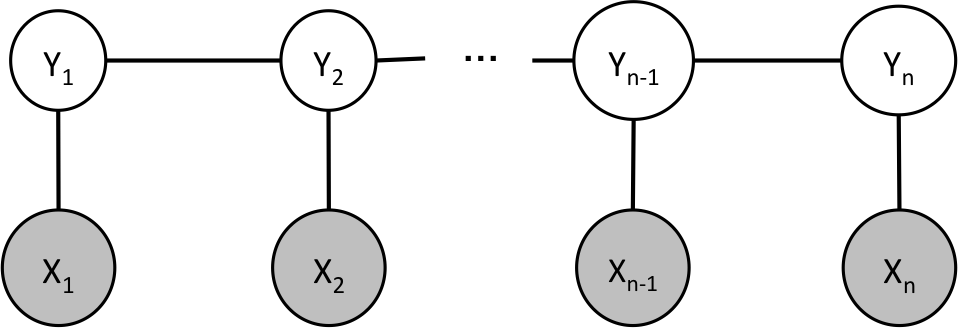
\includegraphics[width=90mm]{3_1.png}
\caption{Graphical model corresponding to the conditional distribution}
\label{meanfieldmodel}
\end{figure}


% 2
\item
We will define two features $f_1(x_i,y_i,y_{i-1})$, $f_2(x_i,y_i,y_{i-1})$ as follows:

\begin{equation*}
f_1(x_i,y_i,y_{i-1})=\begin{cases}
    1, & \text{if $(x_i,y_i,y_{i-1})=(White, I, I)$}.\\
    0, & \text{otherwise}.
  \end{cases}
\end{equation*}

\begin{equation*}
f_2(x_i,y_i,y_{i-1})=\begin{cases}
    1, & \text{if $(x_i,y_i,y_{i-1})=(back, O, O)$}.\\
    0, & \text{otherwise}.
  \end{cases}
\end{equation*}

We expect $f_1$ to be associated with a positive weight $w_1$ because it represents a structural case where the feature only has a non-zero value for when the $y_i$ value corresponds to a case where $x_i$ is a NP.
In an analogous way, we expect $f_2$ to be associated with a negative weight $w_2$ because it represents a structural case where the feature only has a non-zero value for when the $y_i$ value corresponds to a case where $x_i$ is not a NP.

% 3
\item
In order to solve this question, we can refer to sections 6 and 7 on \cite{crf}. Basically, we use the idea of representing the CRF transition probabilities as matrices, and then take advantage of the graphical structure and use the idea similar to that of message passing through the definition of forward and backward vectors and dynamic programming to make this computation feasible in a polynomial complexity. 

We start by defining one matrix $M_i(x)$ of size $|\mathcal{L}|\times|\mathcal{L}|$ for each position $i$, such that its elements are given by

\begin{equation*}
M_i(y',y|{\bf x}) = exp\left(\sum_j w_jf_j(y',y,{\bf x},i)\right)
\end{equation*}

such that

\begin{equation*}
M_i({\bf y}|{\bf x},{\bf w}) = \frac{1}{Z({\bf x})}\prod_{i=1}^{n+1} M_i(y_{i-1},y_i|{\bf x})
\end{equation*}

We then define the forward and backward vectors (reap. $\alpha_i(x)$ and $\beta_i(x)$) as below:

\begin{equation*}
\alpha_0(y|{\bf x})=\begin{cases}
    1, & \text{if $y=start$}.\\
    0, & \text{otherwise}.
  \end{cases}
\end{equation*}

\begin{equation*}
\alpha_i({\bf x})^T = \alpha_{i-1}({\bf x})^TM_i({\bf x})
\end{equation*}

\begin{equation*}
\beta_{n+1}(y|{\bf x})=\begin{cases}
    1, & \text{if $y=stop$}.\\
    0, & \text{otherwise}.
  \end{cases}
\end{equation*}

\begin{equation*}
\beta_i({\bf x})^T = M_{i+1}({\bf x})\beta_{i+1}({\bf x})
\end{equation*}

As a consequence, we are able to compute the probability that a subsequence ${x_i,\dots,x_{i+k}}$ is NP by computing the joint probability using the matrix multiplication and then multiplying the result on the left and on the right by resp. the backward and the forward vectors, which can be interpreted as the message with the marginalization over the remaining variables with indexes resp. smaller and larger than the indexes of the specified subsequence. Mathematically, 

\begin{equation*}
P(y_i = B, y_{i+1} = I, \dots, y_{i+k} =I) = \frac{1}{Z(x)}\alpha_{i-1} M_{i-1}(B, I) \prod_{j=i+1}^{i+k} M_j(I, I) \beta_{i+k}^T
\end{equation*}


% 4
\item
By definition, we have
\begin{equation*}
\mathcal{L}(w) = \sum_{({\bf x},{\bf y})\in\mathcal{D}} \left\{ {\bf w}^T \sum_{i=1}^{|{\bf x}|}f(x_i,y_i,y_{i-1}) - \log Z({\bf x}, {\bf w}) \right\}
\end{equation*}

By taking the partial derivative w.r.t. ${\bf w}$ we get:

\begin{equation*}
\begin{split}
\frac{\partial\mathcal{L}(w)}{\partial w} &= \frac{\partial}{\partial w}\sum_{({\bf x},{\bf y})\in\mathcal{D}} \left\{ {\bf w}^T \sum_{i=1}^{|{\bf x}|}f(x_i,y_i,y_{i-1}) - \log Z({\bf x}, {\bf w}) \right\}\\
&= \sum_{({\bf x},{\bf y})\in\mathcal{D}} \left\{ \sum_{i=1}^{|{\bf x}|}f(x_i,y_i,y_{i-1}) - \frac{\partial}{\partial w} \log Z({\bf x}, {\bf w}) \right\}\\
&= \sum_{({\bf x},{\bf y})\in\mathcal{D}} \left\{ \sum_{i=1}^{|{\bf x}|}f(x_i,y_i,y_{i-1}) - \frac{1}{Z({\bf x}, {\bf w})}\frac{\partial}{\partial w} Z({\bf x}, {\bf w}) \right\}\\
&= \sum_{({\bf x},{\bf y})\in\mathcal{D}} \left\{ \sum_{i=1}^{|{\bf x}|}f(x_i,y_i,y_{i-1}) - \frac{1}{Z({\bf x}, {\bf w})}\frac{\partial}{\partial w} \sum_{y'\in\mathcal{L}^n}exp\left({\bf w}^T \sum_{i=1}^{|{\bf x}|}f(x_i,y'_i,y'_{i-1})\right) \right\}\\
&= \sum_{({\bf x},{\bf y})\in\mathcal{D}} \left\{ \sum_{i=1}^{|{\bf x}|}f(x_i,y_i,y_{i-1}) - \sum_{y'\in\mathcal{L}^n}\frac{1}{Z({\bf x}, {\bf w})} exp\left({\bf w}^T \sum_{i=1}^{|{\bf x}|}f(x_i,y'_i,y'_{i-1})\right)\sum_{i=1}^{|{\bf x}|}f(x_i,y'_i,y'_{i-1}) \right\}\\
&= \sum_{({\bf x},{\bf y})\in\mathcal{D}} \left\{ \sum_{i=1}^{|{\bf x}|}f(x_i,y_i,y_{i-1}) - \sum_{y'\in\mathcal{L}^n}p(y'|x,w) \sum_{i=1}^{|{\bf x}|}f(x_i,y'_i,y'_{i-1}) \right\}\\
&= \sum_{({\bf x},{\bf y})\in\mathcal{D}} \left\{ \sum_{i=1}^{|{\bf x}|}f(x_i,y_i,y_{i-1}) - \mathbb{E}_{p(y'|x,w)}\left[ \sum_{i=1}^{|{\bf x}|}f(x_i,y'_i,y'_{i-1})\right] \right\}\\
&= \sum_{({\bf x},{\bf y})\in\mathcal{D}} \left\{ \sum_{i=1}^{|{\bf x}|} \left\{f(x_i,y_i,y_{i-1}) - \mathbb{E}_{p(y'|x,w)}\left[f(x_i,y'_i,y'_{i-1})\right] \right\}\right\}
\end{split}
\end{equation*}

% 5
\item
We wish to efficiently compute
\begin{equation*}
\sum_{i=1}^{|{\bf x}|}\mathbb{E}_{p(y'|x,w)}\left[ f(x_i,y'_i,y'_{i-1})\right]
\end{equation*}

But we know that

\begin{equation*}
\begin{split}
\sum_{i=1}^{|{\bf x}|}\mathbb{E}_{p(y'|x,w)}\left[ f(x_i,y'_i,y'_{i-1})\right] &= \sum_{i=1}^{|{\bf x}|}\sum_{y'\in\mathcal{L}^n}{p(y'|x,w)}f(x_i,y'_i,y'_{i-1})\\
&= \sum_{i=1}^{|{\bf x}|}\sum_{y'\in\mathcal{L}^n}{\frac{1}{Z({\bf x}, {\bf w})}}exp\left({\bf w}^T \sum_{i=1}^{|{\bf x}|}f(x_i,y'_i,y'_{i-1})\right)f(x_i,y'_i,y'_{i-1})\\
&=  \sum_{i=1}^{|{\bf x}|}\sum_{y'\backslash y'_i,y'_{i-1}}\sum_{y'_i,y'_{i-1}}f(x_i,y'_i,y'_{i-1}) \frac{1}{Z({\bf x}, {\bf w})}exp\left({\bf w}^T \sum_{i=1}^{|{\bf x}|}f(x_i,y'_i,y'_{i-1})\right)\\
&=  \sum_{i=1}^{|{\bf x}|}\sum_{y'_i,y'_{i-1}}f(x_i,y'_i,y'_{i-1}) \sum_{y'\backslash y'_i,y'_{i-1}}\frac{1}{Z({\bf x}, {\bf w})}exp\left({\bf w}^T \sum_{i=1}^{|{\bf x}|}f(x_i,y'_i,y'_{i-1})\right)\\
&=  \sum_{i=1}^{|{\bf x}|}\sum_{y'_i,y'_{i-1}}f(x_i,y'_i,y'_{i-1}) p(y'_i,y'_{i-1}|x,w)
\end{split}
\end{equation*}

But $f(x_i,y'_i,y'_{i-1})$ is easily computable and from part (3) we can compute $p(y'_i,y'_{i-1}|x,w)$ in polynomial time.

Thus, we are able to compute $\sum_{i=1}^{|{\bf x}|}\mathbb{E}_{p(y'|x,w)}\left[ f(x_i,y'_i,y'_{i-1})\right]$ in polynomial time.


\end{enumerate}


% -------------------------------------------------------
%       Problem 4
% -------------------------------------------------------

\section*{Problem 4}


% PART 1
% -------------------------------------------------------
\subsection*{Part 1}

\begin{enumerate}

% 1.1
\item
We first observe that each instance is drawn independently from $\mathcal{N}(\mu,\Sigma)$ where $\Theta = \Sigma^{-1}$.
According to the question notation, $x_i$ is a row vector. We'll follow this notation.
Thus,
\begin{equation*}
\begin{split}
l(\Theta;x_1,\dots,x_n) &= \log p(x_1,\dots,x_n|\Theta)\\
&= \sum_{i=1}^{n} \log p(x_i |\Theta)\\
&= - \sum_{i=1}^{n} \frac{1}{2}\log(2\pi)^p + \sum_{i=1}^{n}\frac{1}{2}\log \det(\Sigma)^{-1} - \sum_{i=1}^{n}\frac{1}{2}x_i\Sigma^{-1} x_i^T\\
&\propto \sum_{i=1}^{n}\log \det(\Sigma)^{-1} - \sum_{i=1}^{n}x_i\Theta x_i^T\\
&= n\log \det(\Theta) - \sum_{i=1}^{n}x_i\Theta x_i^T\\
&\propto \log \det(\Theta) - \frac{1}{n}\sum_{i=1}^{n}x_i\Theta x_i^T\\
\end{split}
\end{equation*}

So far, we've only used the fact that the inverse of the determinant is equal to the determinant of the inverse and that the points are independently drawn form a same multivariate normal distribution.

We now have to prove that $\sum_{i=1}^{n}x_i\Theta x_i^T = tr(X^TX\Theta)$. Let's start by computing $tr(X^TX\Theta)$.

Let's call $A = X^TX$, $M\in\mathbb{R}^{p\times p}$, with elements $A_{ij}$. By the definition of matrix product, we have

\begin{equation*}
A_{ij} = \sum_{k=1}^n x_{ki}x_{kj}
\end{equation*}

Thus, if we call $B = A\Theta$, $B\in\mathbb{R}^{p\times p}$, with elements $B_{xy}$, we have

\begin{equation*}
B_{xy} = \sum_{l=1}^p A_{xl}\Theta_{ly} = \sum_{l=1}^p\sum_{k=1}^n x_{kx}x_{kl}\Theta_{ly}
\end{equation*}


By definition, if $B = X^TX\Theta$, $B\in\mathbb{R}^{p\times p}$, with elements $B_{ij}$, then

\begin{equation*}
tr(X^TX\Theta) = tr(B) = \sum_{i=1}^p B_{ii} = \sum_{i=1}^p\sum_{l=1}^p\sum_{k=1}^n x_{ki}x_{kl}\Theta_{li}
\end{equation*}

Now let's compute $\sum_{k=1}^{n}x_k\Theta x_k^T$ and show that it yields the same expression. 

Let $K_k = x_k\Theta$,  $K_k\in\mathbb{R}^{1\times p}$, with elements $K_{k,1i}$. Thus,

\begin{equation*}
K_{k,1i} = \sum_{l=1}^p x_{kl}\Theta_{li}
\end{equation*}

Back to the main expression, we have

\begin{equation*}
\sum_{k=1}^{n}x_k\Theta x_k^T = \sum_{k=1}^{n}K_{k} x_k^T = \sum_{k=1}^{n}\sum_{i=1}^{p} K_{k,1i} x_{ki} = \sum_{k=1}^{n}\sum_{i=1}^{p} \sum_{l=1}^p x_{kl}\Theta_{li} x_{ki} 
\end{equation*}

Thus,

\begin{equation*}
\sum_{i=1}^{n}x_i\Theta x_i^T = tr(X^TX\Theta)
\end{equation*}

And finally

\begin{equation*}
l(\Theta;x_1,\dots,x_n) \propto \log \det(\Theta) - \frac{1}{n}tr(X^TX\Theta)
\end{equation*}


% 1.2
\item We now use the previous expression to compute the maximum likelihood estimate

\begin{equation*}
\hat{\Theta}^{ML} = \arg\max_{\Theta} l(\Theta;x_1,\dots,x_n) = \arg\max_{\Theta} \left(\log \det(\Theta) - tr(S\Theta)\right)
\end{equation*}

From matrix calculus, we know:

\begin{itemize}
\item Derivative of the determinant:
\begin{equation*}
\frac{\partial\det\Theta}{\partial \Theta} = adjunct(\Theta) = \det(\Theta) \Theta^{-1} = \det(\Theta) \Sigma
\end{equation*}
\item Derivative of product in the trace 
\begin{equation*}
\frac{\partial tr(S\Theta)}{\partial \Theta} = S
\end{equation*}
\end{itemize}

Thus, by deviating the likelihood expression and setting it to zero, we get:

\begin{equation*}
\frac{\partial\log\det\Theta}{\partial \Theta} - \frac{\partial tr(S\Theta)}{\partial \Theta} = 0
\end{equation*}

Using chain rule, we get

\begin{equation*}
\frac{1}{\det\Theta}\frac{\partial\det\Theta}{\partial \Theta} - \frac{\partial tr(S\Theta)}{\partial \Theta} = 0
\end{equation*}

Thus,

\begin{equation*}
\frac{1}{\det\Theta}\det(\Theta)\Sigma - S = 0
\end{equation*}

Finally,

\begin{equation*}
\hat{\Theta}^{ML} = S = \frac{1}{n}X^TX
\end{equation*}

%1.3
\item
If the sample covariance matrix is not positive definite, we cannot compute MLE. And even if it can be computed, that method tends to overfit data (will have high variance). It is usually preferable to have some sort of regularization (as we'll see below).

\end{enumerate}

\newpage
% PART 2
% -------------------------------------------------------
\subsection*{Part 2}

\begin{enumerate}

% 2.1
\item
See submitted code

% 2.2
\item
See submitted code

% 2.3
\item
Results:
%NEIGHBOR SELECTION
\begin{figure}[ht!]
\centering

\begin{subfigure}{.5\textwidth}
  \centering
  
\includegraphics[width=.8\linewidth]{ns_0.png}
  \caption{Neighbor Selection $\lambda=0$}
\end{subfigure}%
\begin{subfigure}{.5\textwidth}
  \centering
  
\includegraphics[width=.8\linewidth]{ns_1.png}
  \caption{Neighbor Selection $\lambda=1$}
\end{subfigure}

\begin{subfigure}{.5\textwidth}
  \centering
  
\includegraphics[width=.8\linewidth]{ns_5.png}
  \caption{Neighbor Selection $\lambda=5$}
\end{subfigure}%
\begin{subfigure}{.5\textwidth}
  \centering
  
\includegraphics[width=.8\linewidth]{ns_10.png}
  \caption{Neighbor Selection $\lambda=10$}
\end{subfigure}

\begin{subfigure}{.5\textwidth}
  \centering
  
\includegraphics[width=.8\linewidth]{ns_30.png}
  \caption{Neighbor Selection $\lambda=30$}
\end{subfigure}%


\end{figure}

%GLASSO
\begin{figure}[ht!]
\centering
\begin{subfigure}{.5\textwidth}
  \centering
  
\includegraphics[width=.8\linewidth]{glasso_0_00.png}
  \caption{Graphical Lasso $\lambda=0.00$}
\end{subfigure}%
\begin{subfigure}{.5\textwidth}
  \centering
  
\includegraphics[width=.8\linewidth]{glasso_0_20.png}
  \caption{Graphical Lasso $\lambda=0.20$}
\end{subfigure}

\begin{subfigure}{.5\textwidth}
  \centering
  
\includegraphics[width=.8\linewidth]{glasso_0_38.png}
  \caption{Graphical Lasso $\lambda=0.38$}
\end{subfigure}%
\begin{subfigure}{.5\textwidth}
  \centering
  
\includegraphics[width=.8\linewidth]{glasso_0_40.png}
  \caption{Graphical Lasso $\lambda=0.40$}
\end{subfigure}

\begin{subfigure}{.5\textwidth}
  \centering
  
\includegraphics[width=.8\linewidth]{glasso_0_41.png}
  \caption{Graphical Lasso $\lambda=0.41$}
\end{subfigure}%
\begin{subfigure}{.5\textwidth}
  \centering
  
\includegraphics[width=.8\linewidth]{glasso_0_80.png}
  \caption{Graphical Lasso $\lambda=0.80$}
\end{subfigure}

\end{figure}


\end{enumerate}




\newpage
% -------------------------------------------------------
%       Bibliography
% -------------------------------------------------------

\begin{thebibliography}{1}

  \bibitem{lda} Blei, David M., Andrew Y. Ng, and Michael I. Jordan. "Latent dirichlet allocation." the Journal of machine Learning research 3 (2003): 993-1022.

  \bibitem{crf} Wallach, Hanna M. "Conditional random fields: An introduction." Technical Reports (CIS) (2004): 22.
  
  \bibitem{glasso} Glasso Algorithm - http://publish.illinois.edu/xiaohuichen/

\end{thebibliography}




\end{document}